\section*{Exercice 175 -- Liaison équivalente}
\setcounter{exo}{0}
\ifprof
\else

\begin{center}
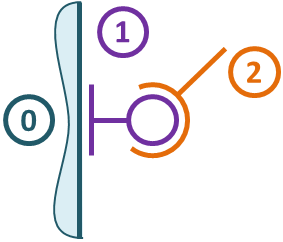
\includegraphics[width=.5\linewidth]{042_01}
%\textit{}
\end{center}

\subparagraph{}
\textit{Paramétrer le schéma cinématique.}


\subparagraph{}
\textit{Déterminer la liaison équivalente entre 0 et 2.}


